%!TEX root = ../../14-icra-RealTimeNMPC.tex

\tikzstyle{block} = [draw, fill=blue!20, rectangle,
    minimum height=2em, minimum width=5em, align=center]
\tikzstyle{sum} = [draw, fill=blue!20, circle, node distance=1cm]
\tikzstyle{input} = [coordinate]
\tikzstyle{output} = [coordinate]
\tikzstyle{pinstyle} = [pin edge={to-,thin,black}]

% The block diagram code is probably more verbose than necessary
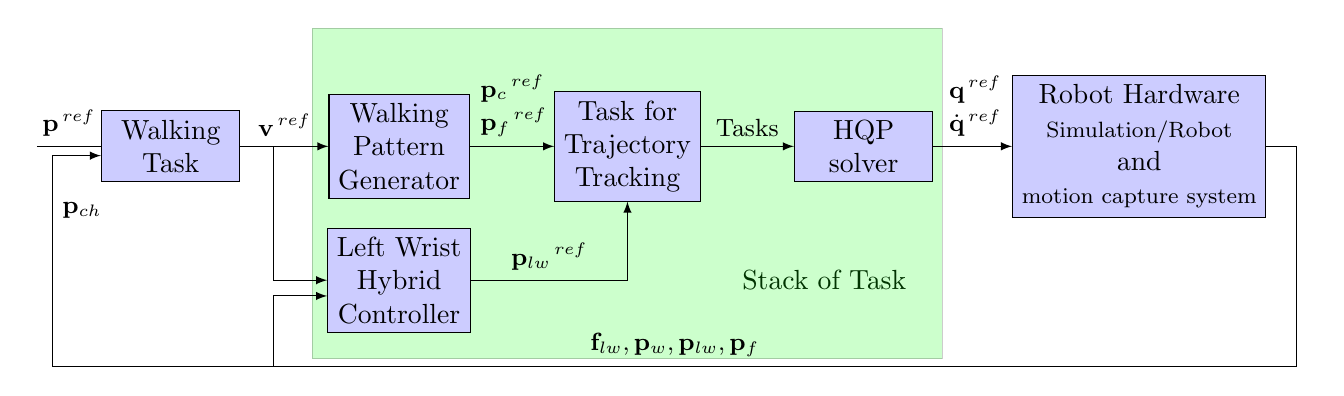
\begin{tikzpicture}[auto, node distance=2cm,>=latex]

    % We start by placing the blocks
    \node [input]  at (0.0, 0.0) (input)  {};
    \node [input]  at (3, 0.0) (velocity) {};
    \node [input]  at (0.2, -2.8) (feedback)  {};
    \node [input]  at (16, -2.8) (feedback2)  {};
    \node []    at ( 0.0, 0.0) (sumin)  {};
    %\node [output]    at ( 15, 0.0) (sumout) {};
    \draw [fill=green,opacity=.2,text opacity=1] (3.5,1.5) rectangle (11.5,-2.7);
    \node at(10,-1.7) {\textcolor{green!20!black!100}{Stack of Task}};

    \node [block] at (4.6,-1.7) (lwc) {
        Left Wrist\\
        Hybrid\\
        Controller        
    };

    \node [block] at (1.7,0.0) (walking) {
        Walking \\
        Task    
    };

    \node [block] at (4.6,0) (wpg) {
        Walking\\
        Pattern\\
        Generator
    };
%    \node [block] at (4.2,0) (dyn) {
%        Dynamic\\
%        Filter
%    };
    \node [block] at (7.5,0) (ttt) {
        Task for\\
        Trajectory\\
        Tracking
    };
    
    \node [block] at (10.5,0) (qp) {
        HQP\\
        solver
    };

    \node [block] at (14.0, 0) (system) {
    		Robot Hardware\\
    		{\footnotesize Simulation/Robot}\\
    		and\\
    		{\footnotesize motion capture system}
    	};

    % PATHS
    	% Forward chaine
    \draw [draw,-] (input) -- node {\small ${\mathbf{p}}^{\,{\text {ref}}}$} (walking);
    
    \draw [draw,->] (walking) -- node {\small ${\mathbf v}^{\,{\text{ref}}}$} (wpg);
%    \draw [draw,- ] (walking) -- node {} (velocity);
    \draw [draw,->] (velocity) |- node {} (lwc);
%    \draw [->] (wpg) -- node {\small $c^{ref},f^{ref}$} (dyn);
%    \draw [->] (dyn) -- node {\small $\tilde{c}^{\,ref},f^{ref}$} (sot);
    \draw [->] (wpg) -- node [text width=0.8cm]{\small ${\mathbf{p}_c}^{\,{\text {ref}}}$ ${\mathbf{p}_f}^{\,{\text {ref}}}$} (ttt);
    \draw [->] (ttt) -- node [text width=0.8cm]{
    \small Tasks
    } (qp);
    \draw [->] (qp) -- node [text width=0.6cm]{\small ${\mathbf q}^{\,{\text{ref}}}$ $\dot{{\mathbf q}}^{\,{\text{ref}}}$} (system);
    
    \draw [->] (lwc) -| node [near start, above]{\small ${\mathbf{p}_{lw}}^{\,{\text {ref}}}$} (ttt);
    %\draw [->] (system) -- node {} (sumout);

    % Feedback chaine
%    \draw [- ] (dyn)      -| node {} (feedback);
%    \draw [->] (feedback) -| node {} (wpg);
    
    \draw [- ] (system.east)    -| node {} (feedback2);
    \draw [- ] (feedback2)  -- node [above]{\small $\mathbf{f}_{lw},\mathbf{p}_{w},\mathbf{p}_{lw},\mathbf{p}_{f}$} (feedback);
    \draw [->] (3.0,-2.8) |- node [near start, above]{} ([yshift=-0.2cm]lwc.west);
    \draw [->] (feedback) |- node [below=0.7cm, right]{\small $\mathbf{p}_{ch}$} ([yshift=-0.2cm]walking);

%    \draw [->] (dyn) -| node[above right] {\small $\hat{c}^{\,x,y,\theta}$, $\hat{f}^{\,\,x,y,\theta}$} (wpg);
\end{tikzpicture}
